\RequirePackage{plautopatch}

\documentclass[a4paper,10pt]{ltjsarticle}
\usepackage{luatexja}

\usepackage{geometry}
\usepackage{multicol}
\usepackage{amsmath}
\usepackage{titlesec}
\usepackage{tocloft}
\usepackage{caption}
\usepackage{flushend}
\usepackage{graphicx}
\usepackage{here}
\usepackage{subfig}
\usepackage{multirow}
\usepackage{threeparttable}
\usepackage{tabularx}
\usepackage{enumitem}
\usepackage{url}
\usepackage{booktabs}
\usepackage{array}
\usepackage{mathptmx}



\geometry{
top=20mm,
bottom=20mm,
left=20mm,
right=20mm
}

\setlength{\baselineskip}{14pt}
\setlength{\parindent}{1\zw}

\titleformat{\section}{\large\bfseries}{\thesection.}{1\zw}{}
\titleformat{\subsection}{\large\bfseries}{\thesubsection.}{1\zw}{}
\titleformat{\subsubsection}{\large\bfseries}{\thesubsubsection.}{1\zw}{}

\setcounter{tocdepth}{3}
\makeatletter
\renewcommand{\numberline}[1]{#1.~}
\renewcommand{\cftsecleader}{\cftdotfill{\cftdotsep}}
\renewcommand{\cftsubsecleader}{\hfill}
\renewcommand{\cftsubsubsecleader}{\hfill}
\cftpagenumbersoff{subsection}
\cftpagenumbersoff{subsubsection}
\makeatother

\DeclareCaptionFont{designatedFont}{\fontsize{10.5pt}{14pt}\selectfont}
\captionsetup{font=designatedFont}

\begin{document}
\fontsize{10.5pt}{14pt}\selectfont

\tableofcontents
\thispagestyle{empty}
\clearpage

\setcounter{page}{1}
% ---------
% 本文開始
% ---------
\section{はじめに}
ドローンを用いたネットワークにおいて,オーバーリーチの問題を解決するために送信信号の届く中継局まで一度に中継するCTR(Cooperation Through Relay)方式[1]を提案している. 本稿では,提案手法において干渉/誤りが生じた際のスループット特性を従来方式と比較し評価する.


\begingroup
\renewcommand{\rmdefault}{ptm} % Times New Roman に変更
\begin{table}[h]
  \caption{Modulation and Coding Table}
  \centering
  \renewcommand{\arraystretch}{1.2}
  \begin{tabular}{c c c c}
    \toprule
    TR [Mbps] & Modulation & Coding & Rmin [dBm] \\ 
    \midrule
    6  & BPSK  & 1/2  & -82 \\
    9  & BPSK  & 3/4  & -81 \\
    12 & QPSK  & 1/2  & -79 \\
    18 & QPSK  & 3/4  & -77 \\
    24 & 16QAM & 1/2  & -74 \\
    36 & 16QAM & 3/4  & -70 \\
    48 & 64QAM & 2/3  & -66 \\
    54 & 64QAM & 3/4  & -65 \\
    \bottomrule
  \end{tabular}
  
  \label{tab:modulation_coding}
\end{table}
\endgroup



\section{従来方式の概要}
図1に従来方式である概要を示す.従来の中継伝送では1ホップずつ中継するが,自由空間では,伝搬損失が少ないため送信信号が中継先のドローン(図1\#3)より遠くのドローン(図1\#4)に到達することで干渉が生じる.そのため,従来方式はオーバーリーチ干渉によってパケットの再送によってチャネルの利用効率が低下する.また,従来方式で干渉が生じ,再送を行う際には,フォールバック制御により伝送レートを下げることでSNR(Signal to Noise Ratio)が低くてもパケットを受信できるようにしているが,伝送レートの低下に伴って送信時間や再送によるオーバヘッドが増加してしまう課題がある.

\begin{figure}[H]
  \centering
  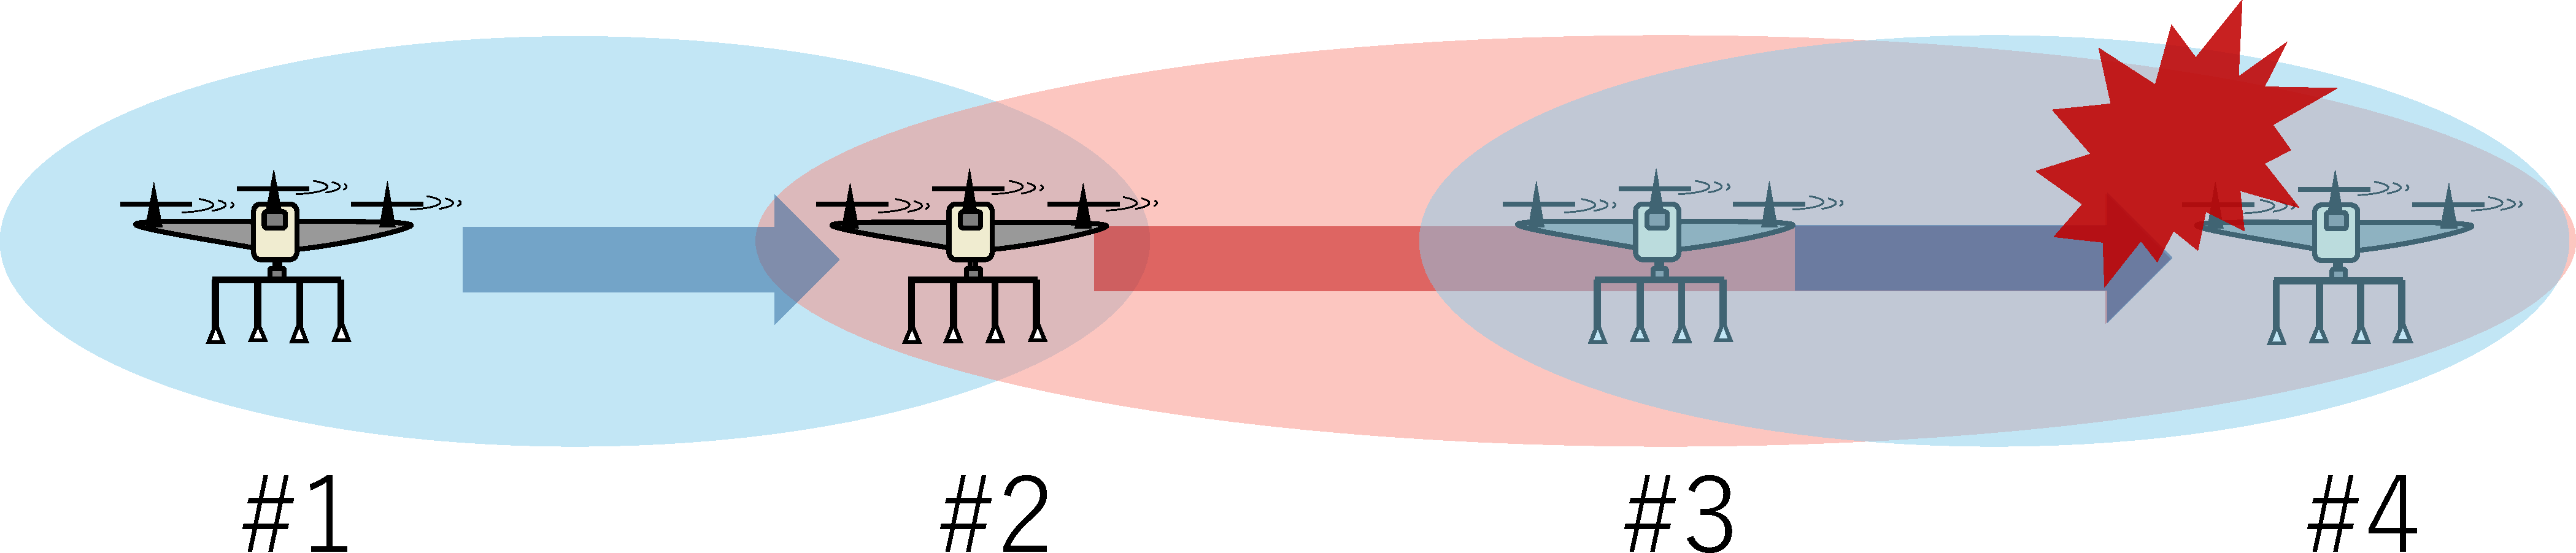
\includegraphics[width=\linewidth]{cenventional_topology.pdf} % 図のファイル名を指定
  \caption{従来の方式の概要}
  \label{fig:従来の方式のトポロジー} % 参照用ラベル
\end{figure}

\section{CTR方式の概要}
オーバリーチ干渉は送信信号が中継局のドローンを超えて他のドローンに干渉することで発生する.そこでCTR方式では直線状に存在する中継局が協調することによってオーバリーチ干渉の問題を解決する.
図2に示すCTR方式は,送信信号の届く範囲の最終中継局(図 1\#4)まで一度に信号を送信し,通信経路の中継局(図1\#3)も協調してパケットを受信する.最終中継局がパケットを正常に受信した場合は,以後,同様の手順で中継する.最終中継局がパケットの受信に失敗した場合は,直線経路の中継局\#3が\#4の代わりに次の中継局へパケットを中継する.そのため従来方式ではオーバーリーチ干渉が生じる環境でもCTR方式ではオーバーリーチ干渉が減り中継ホップ数も減るので中継オーバヘッドも削減することができる.

\begin{figure}[H]
  \centering
  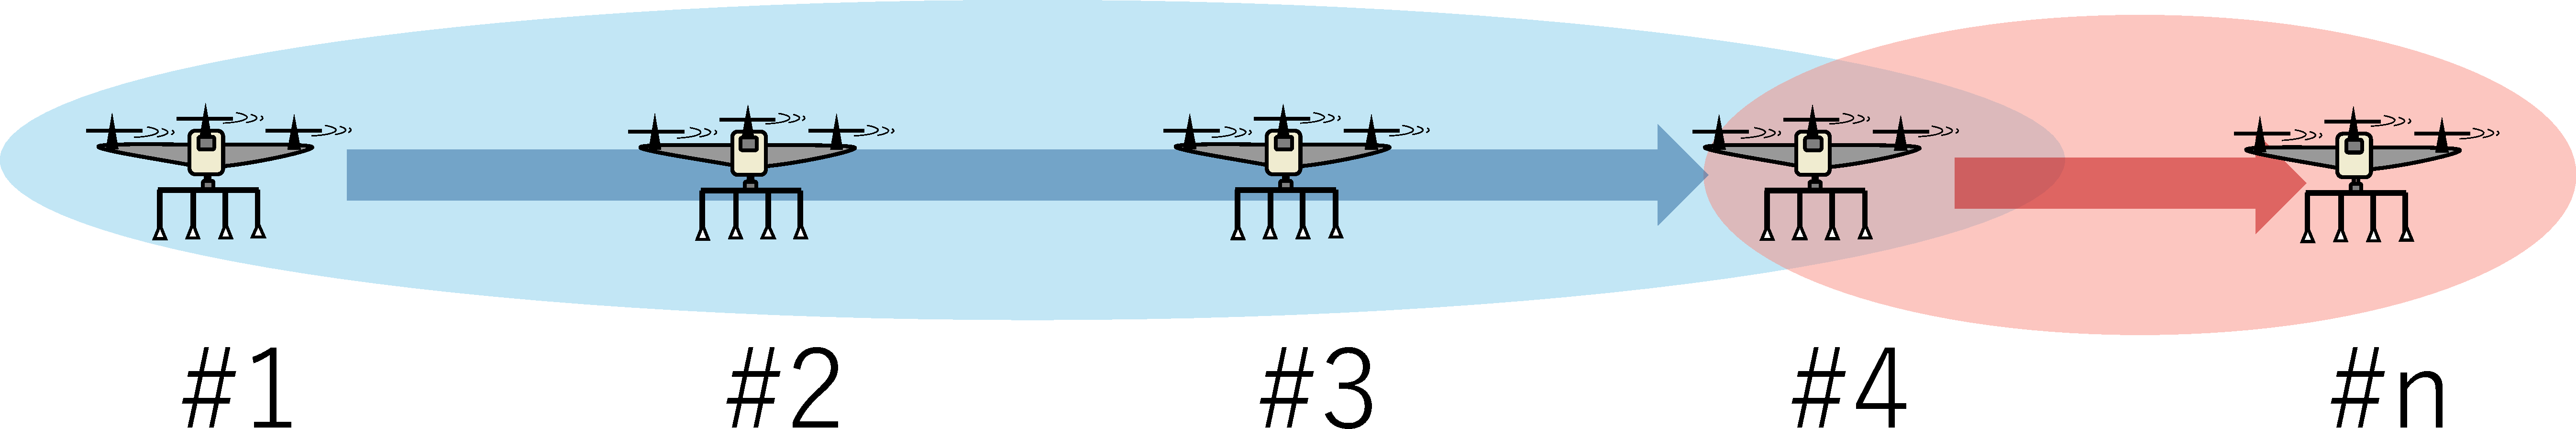
\includegraphics[width=\linewidth]{CTR_topology.pdf} % 図のファイル名を指定
  \caption{CTR方式の概要}
  \label{fig:CTR方式のトポロジー} % 参照用ラベル
\end{figure}

図3にCTR方式の詳細なアクセス制御手順を示す。本方式では、最終中継局がパケットを受信できなかった場合でも中継を継続できる仕組みが導入されている。送信局がランダムなバックオフ時間の後、ACK(Acknowledgement)durationを記述したパケットを送信する.
パケットを受信した中継局は、指定されたACK duration後に送信局へACKを返信する.ACK durationはスロットタイムで区切られ、最終受信中継局が最短のACK durationを持ち、送信局に近づくにつれてスロットタイムが1ずつ増加する設計となっている。
これは送信電力の制御や、各端末のSNR(Signal-to-Noise Ratio)および受信電力閾値に基づく自律的な判断を行い信号が到達する最大範囲を推定することでスロットタイムが適切に設定される仕組みとなっている。
具体的には, 図3\#4がパケットを受信した場合,スロットタイムは受信電力より\#3,\#2の順番で増加し,送信局の\#1にACKを返信すると,経路上の中継局である\#2,\#3はACKの送信待ちをキャンセルする.最終受信中継局(図3\#4)がパケットの受信に失敗した場合は\#3が送信局の\#1 にACKを送信し,\#4の代わりとして中継を続行する.
これにより,従来方式の再送でのオーバーヘッドの増加や,フォールバック制御による伝送レートを低下を防ぐことができる.

\begin{figure}[H]
  \centering
  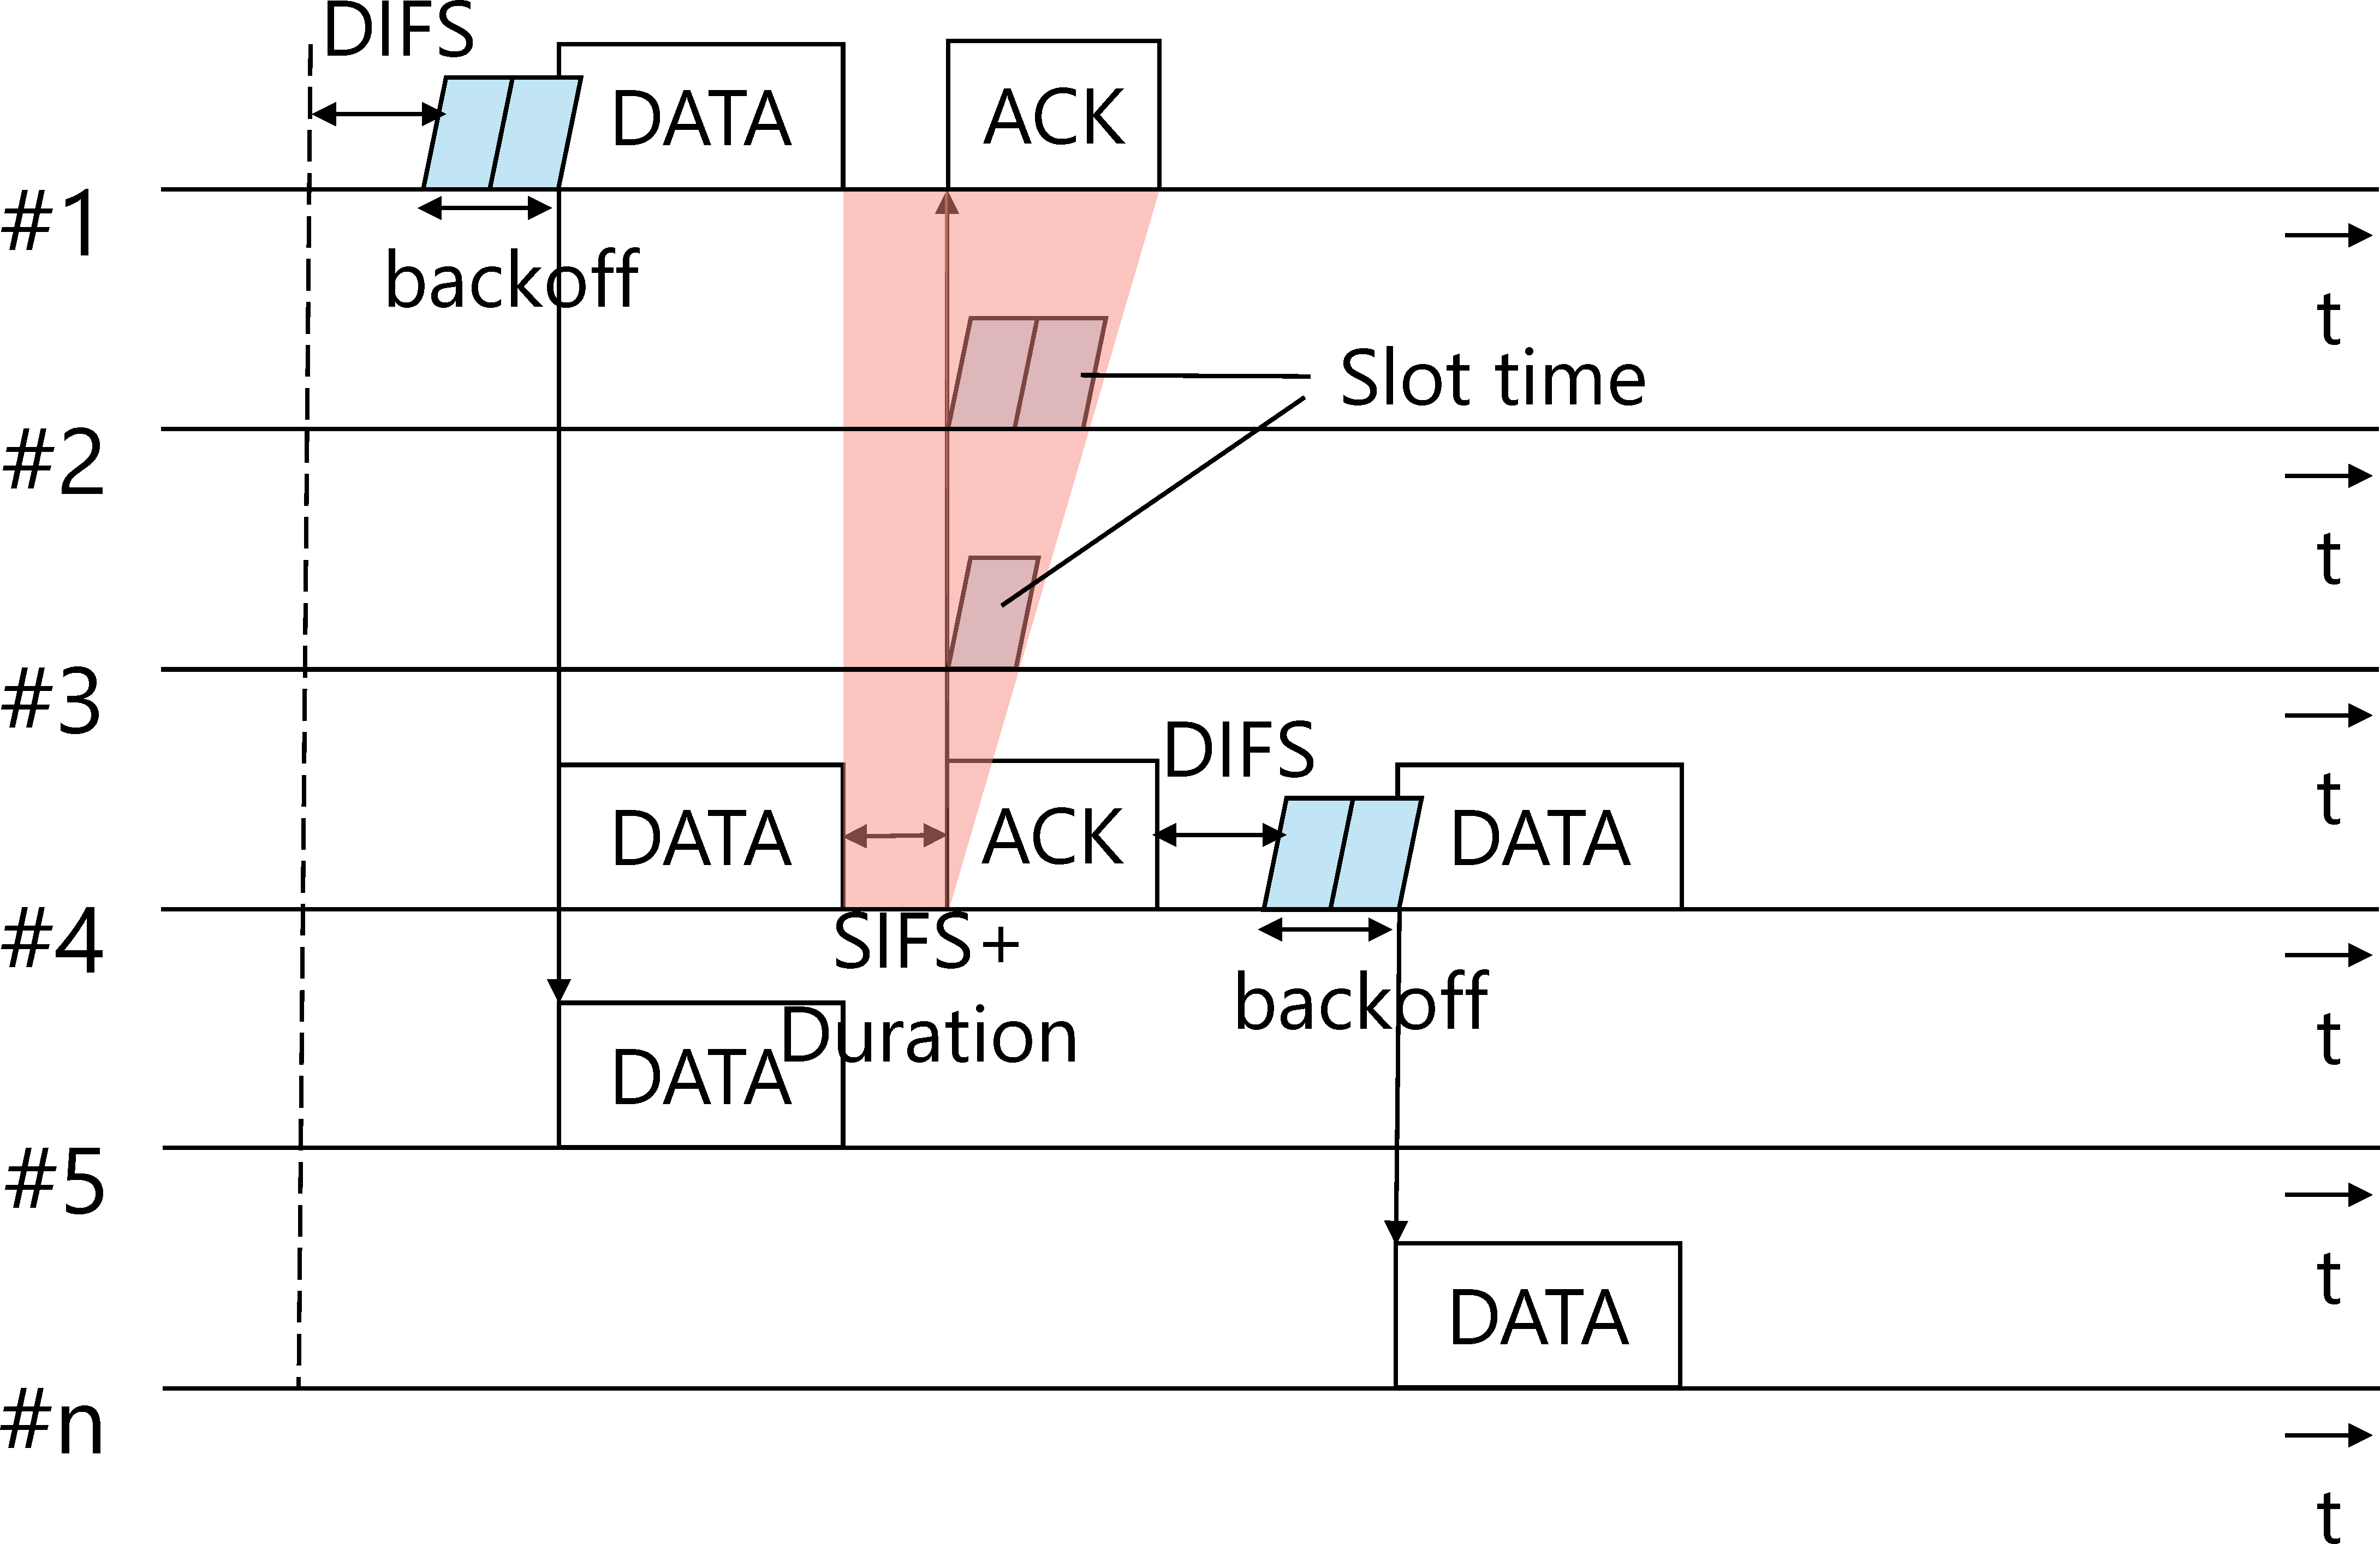
\includegraphics[width=\linewidth]{CTR_accsess.pdf} % 図のファイル名を指定
  \caption{CTR方式のアクセス制御}
  \label{fig:CTR方式のアクセス制御} % 参照用ラベル
\end{figure}

\section{CTR方式の評価}
\subsection{誤りが無い条件でのCTR方式の評価}
CTR方式の特徴である中継局をスルーすることによるスループットの向上を以下の条件で従来方式と比較する.
中継の総伝送距離は1000mとし,50m間隔で直線状に20台のドローンを配置した.アンテナの送受信利得は0dBi,送信電力は10dBmとした.周波数は2.4GHz,伝送レートはIEEE 802.11aを参考にし,伝搬損失は自由空間伝搬損失とした.
評価内容は従来の1ホップ中継(54Mbps) と中継局を2台スルー(24Mbps) した場合,および中継局を3台スルー(18Mbps) した場合におけるスループット特性を確認する.括弧内は使用可能な最も高い伝送レートである.これは受信電力よりIEEE 802.11aのMCS (Modulation and Coding Scheme) indexから選択する.

図4にCTR方式のスループット特性を示す.従来の1ホップ中継と比べてCTR方式で中継局を3台スルーした条件では約2倍のスループットが得られた.
ドローンをスルーする場合は,通信距離が長くなり使用可能な伝送レートが低下するが、アクセス制御やプリアンブル等のオーバヘッドとのトレードオフになる.その結果,ネットワーク全体の通信効率において,中継局を3台スルーする条件が最も高くなることを確認した.

\begin{figure}[H]
  \centering
  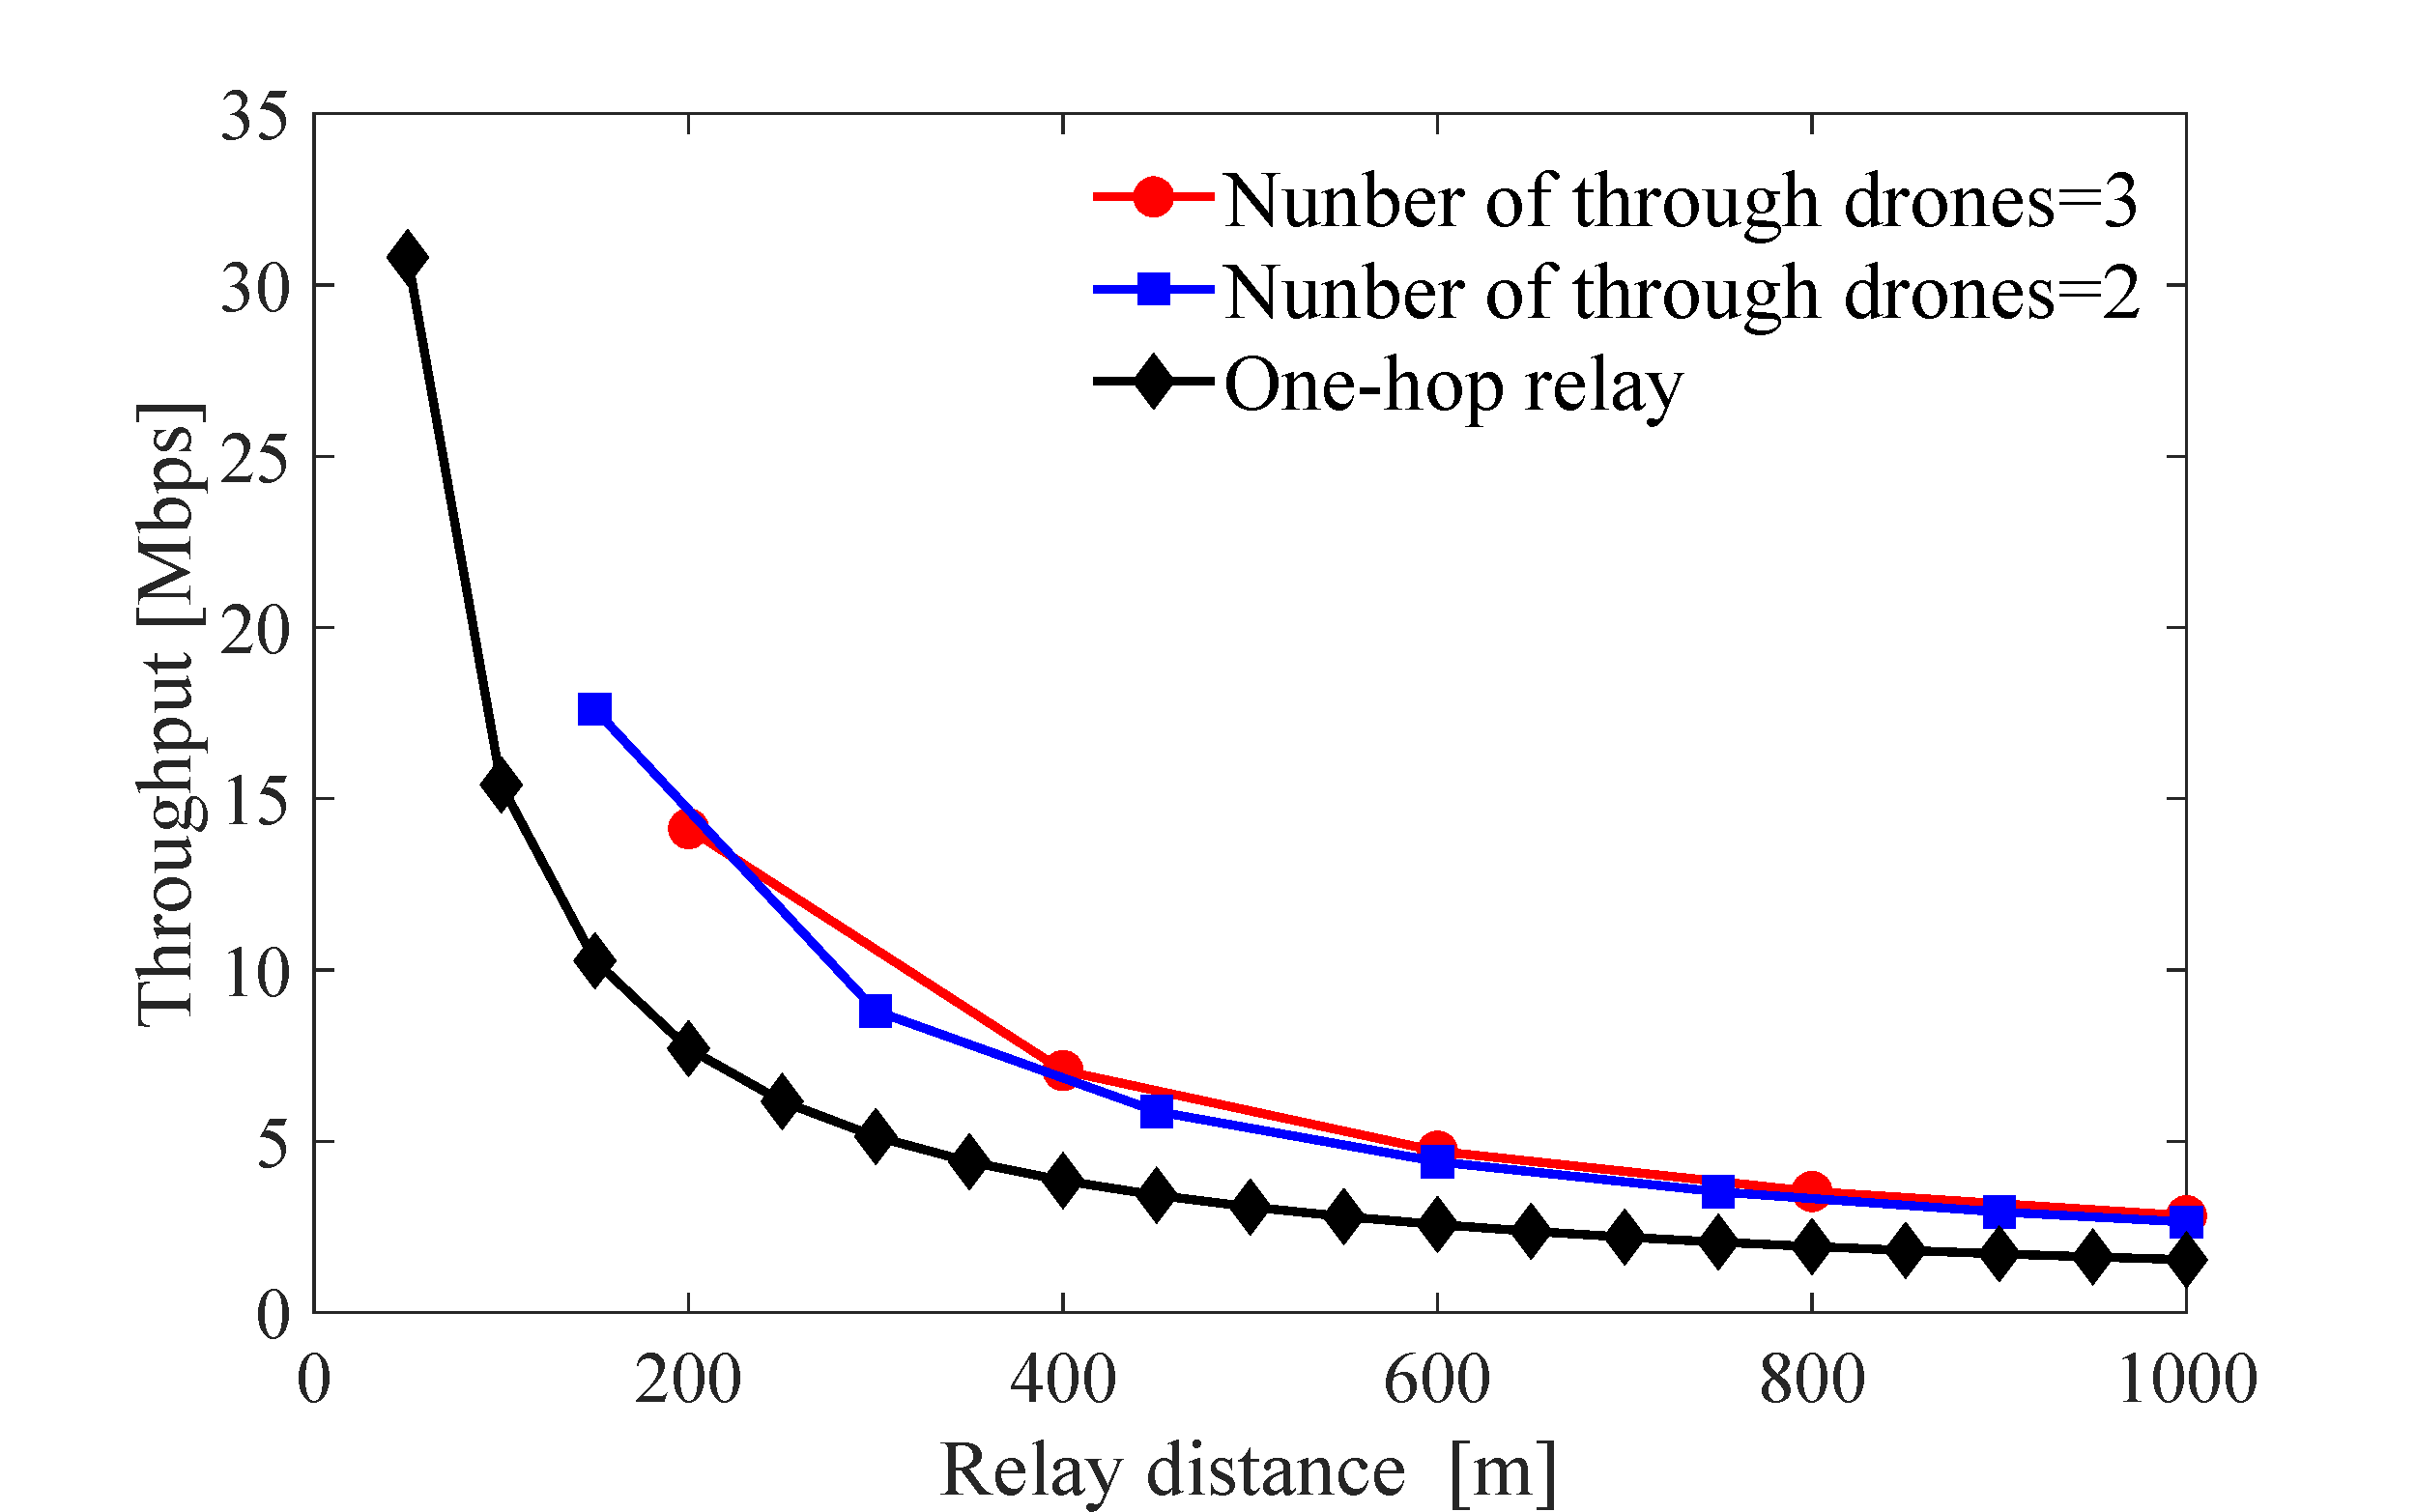
\includegraphics[width=\linewidth]{throughtput_vs_placement_50m_max_distance_3.pdf} % 図のファイル名を指定
  \caption{CTR方式のスループット特性}
  \label{fig:throughput_through} % 参照用ラベル
\end{figure}

\subsection{誤りを生じる条件でのCTR方式の評価}
CTR方式のもう一つの特徴は、中継時に誤りが発生した場合、経路上の中継局が代替して中継を行うことにより、従来方式と比較してスループットが向上する点である。この特性を、4.1の条件に基づいて従来方式と比較する。伝送レートは4.1の評価結果に基づき、18Mbpsとする。誤りが生じた際、従来方式ではフォールバック制御により伝送レートを1つ下の12Mbpsに変更し、その後の再送信は必ず成功するとする。これに対して、CTR方式では、誤りが生じた際、正しく受信できなかった中継局の1つ手前の中継局が必ず代替して中継できるとする.
この時パケットの誤り率を0\%から100\%まで変化させたときの従来方式とCTR方式の1000m地点での最終的なスループット特性を比較した.

図5に誤り率が変化したときスループットを示す.この結果から,誤り率が増加するほど従来方式よりスループットが高くなっているため,従来方式よりもCTR方式は干渉等によって局所的に誤り率が上がる条件(受信局)でも高効率に中継伝送が可能なことを確認した.
また,誤り率が増加するにつれて従来方式とCTR方式のスループットは減少しているが,CTR方式では誤り率によってスループットが緩やかに減少する部分がある.これはパケットの送信回数が関係していると考える.図6には誤り率に対しての平均送信回数を示す.図6より従来方式の送信回数は誤り率に対して線形的に変化しているが,CTR方式の送信回数は線形的には変化していない.
これは,CTR方式で誤りが生じた際に,一つ前の中継局が通信を代替するからで,その結果,パケットの誤り率が増加しても送信回数の増加は緩やかに抑えられる.この送信回数の抑制によりCTR方式のスループットは従来の方式と比較して減少が緩やかになる部分があると考えた.

\begin{figure}[H]
  \centering
  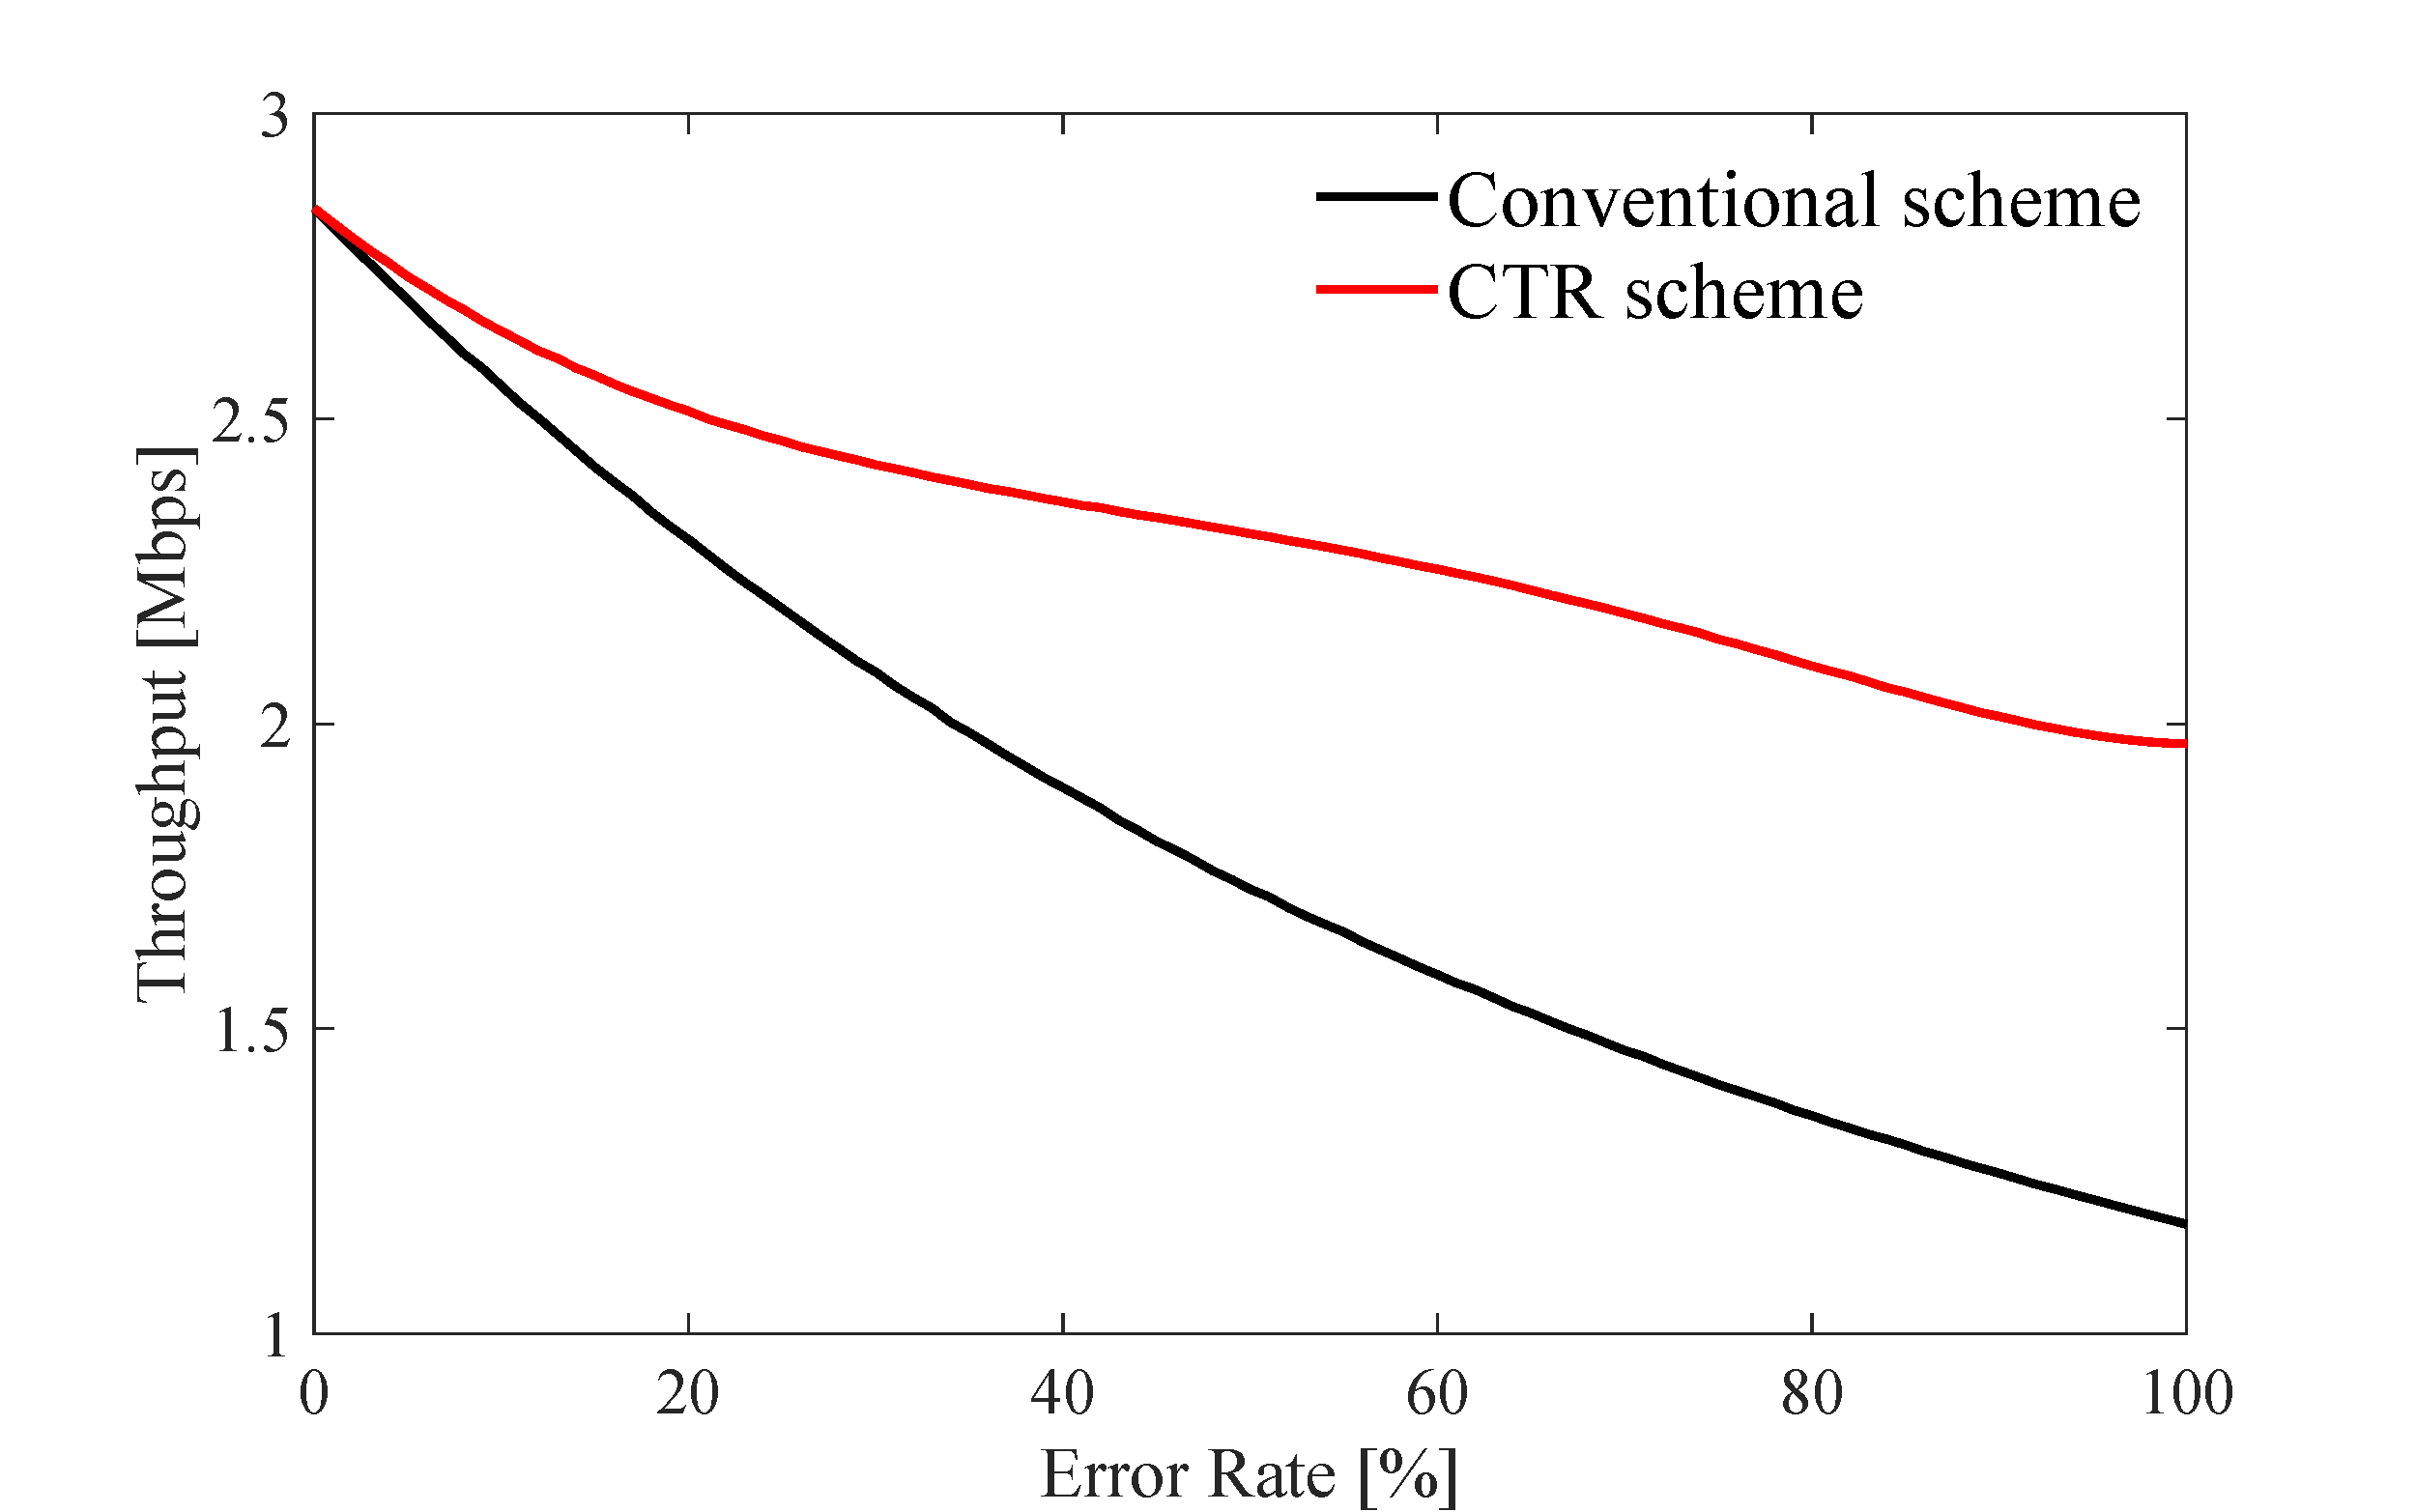
\includegraphics[width=\linewidth]{throughput_probabilistic_retry_v3.pdf} % 図のファイル名を指定
  \caption{誤り率に対するスループット特性}
  \label{fig:throughput_v3} % 参照用ラベル
\end{figure}
\begin{figure}[H]
  \centering
  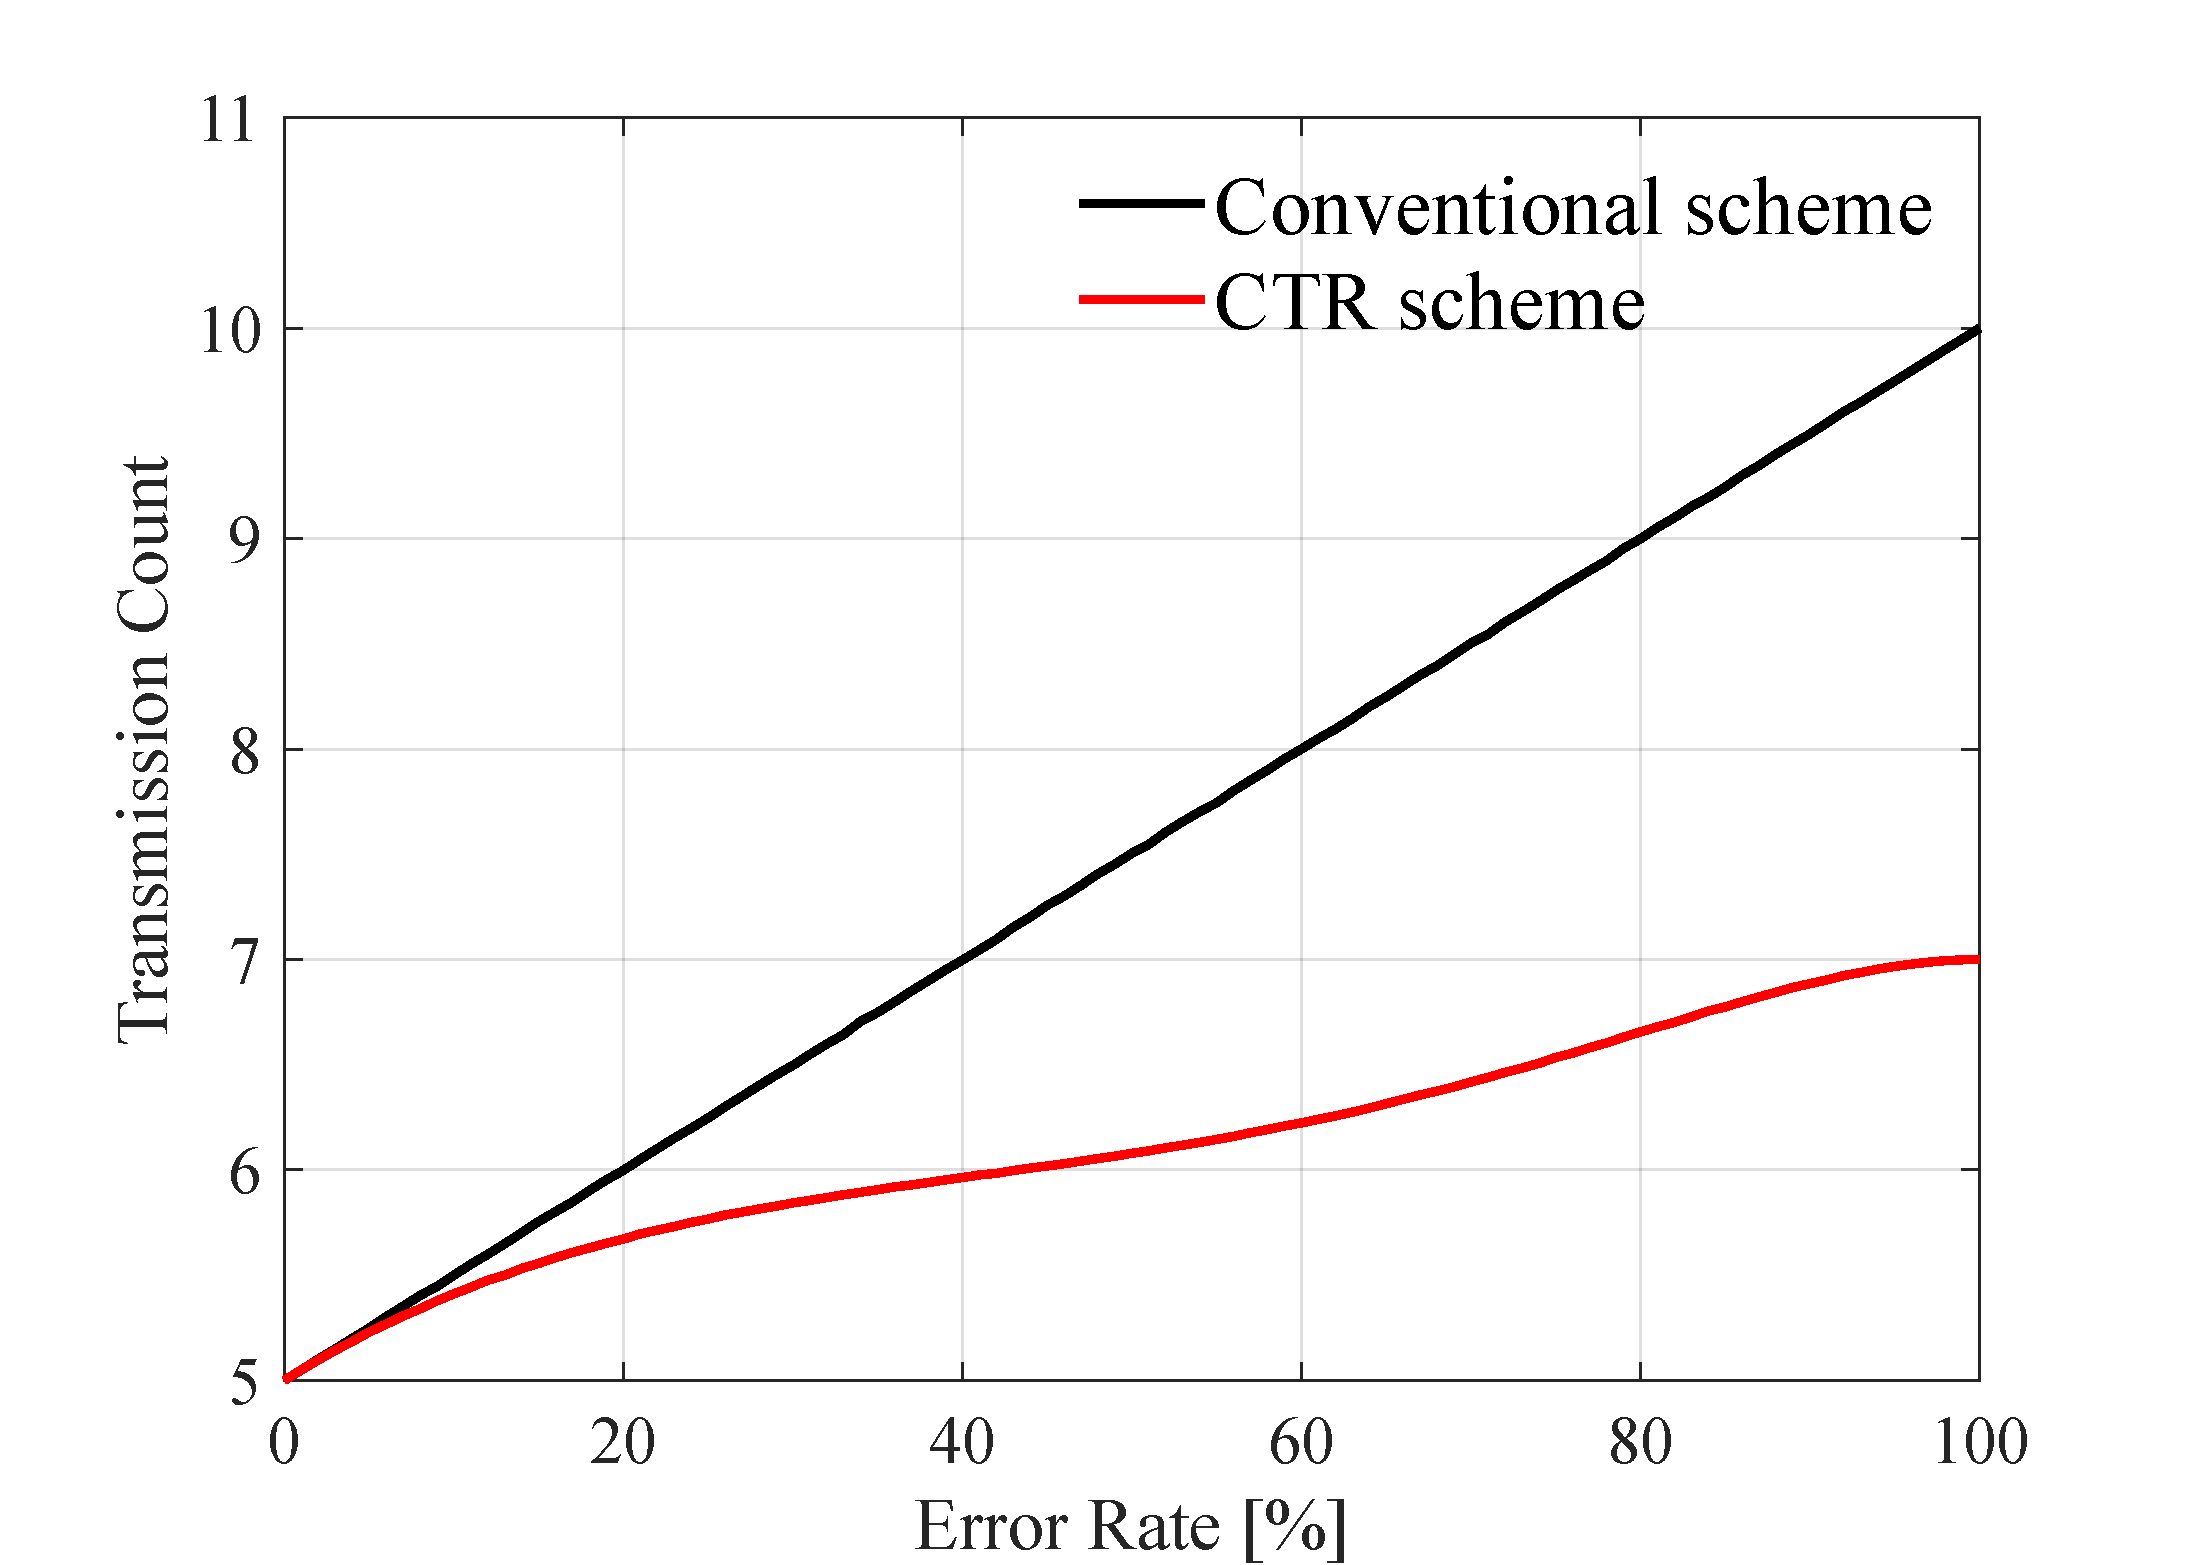
\includegraphics[width=\linewidth]{throughput_probabilistic_retry_v3.1.pdf} % 図のファイル名を指定
  \caption{誤り率に対しての平均送信回数の変化}
  \label{fig:throughput_v3.1} % 参照用ラベル
\end{figure}

\section{まとめ}
本稿では,直線に配置されたドローン中継伝送におけるオーバリーチ干渉の影響を解決するために,送信信号の届く中継局まで一回で中継するCTR方式を検討した.
CTR方式と従来の方式で誤りが生じた場合と生じない場合のスループット特性を計算し比較した.
この結果からいずれの条件でもCTR方式はスループットが従来方式より高いことがわかった.
CTR方式では誤りが発生した場合においても再送信時にフォールバック制御による伝送レートの低下や中継時間の増加を防ぐことができるため、高効率な中継伝送が可能である.

\end{document}